\section{Experimental Evaluations}\label{sec:expts}

We generate synthetic datasets, $D_{\tn{syn}}$ of sizes much smaller than the original training dataset using Algorithms \ref{alg:one} and \ref{alg:two} for supervised regression and offline RL respectively. We evaluate the models trained on them, over the test split of the original dataset in case of supervised regression or the derived policy in the RL environment. \\
\textbf{Baselines}. The following baseline datasets are included as part of our experiments. {\it Full Original}: model trained on the entire original training dataset $D_{\tn{train}}$,  and {\it Random}: model trained on a random sub-sample (of same size as the synthetic dataset) of the original dataset, $D_{\tn{rand}}$. In addition, for supervised regression, {\it Leveraged}: model trained on a leverage score subsample (of same size as the synthetic dataset) of the original dataset, $D_{\tn{lev}}$ (see \cite{drineas2006fast}).




{\bf Supervised Regression Datset Distillation.} We evaluate Algorithm \ref{alg:one} along with the above mentioned baselines on the Wine Quality (\cite{cortez2009modeling} ODbL 1.0 License), 
specifically the included red wine and white wine quality datasets, and the Boston Housing Dataset~\citep{housing}.


The sizes of the synthetic dataset $N_{\tn{syn}}$ we consider are $\{20, 50, 100\}$. The size of $D_{\tn{rand}}$ and $D_{\tn{lev}}$ are the same as $D_{\tn{syn}}$, and is subsampled randomly from $D_{\tn{train}}$. We initialise the convex optimisation of $D_{\tn{syn}}$ with the initial value $D_{\tn{rand}}$. We take $k=100$ random homogeneous linear regressors in Algorithm \ref{alg:one} to find $D_{\tn{syn}}$ and then train a homogenous linear model ($f(\bx) = \br^T\bx$) on the four datasets. 

The mean test loss of models trained on respective datasets (over $10$ trials) are plotted in Figure~\ref{fig:supervised}. Further details of the model training, hyperparameter search are included in Appendix \ref{sec:expts-wine} and Appendix \ref{sec:expts-housing}.

We observe that the homogenous linear models trained on $D_{\tn{syn}}$ performs almost as well as ones trained on $D_{\tn{train}}$, far better than ones trained on $D_{\tn{rand}}$, and better or on par with the models trained on $D_{\tn{lev}}$. This demonstrates the efficacy of our synthetic data generation technique for supervised learning datasets and empirically verifies Theorem~\ref{thm:supervised-distill-1}. We also observe that we perform better than the classical data-reduction technique of leverage score subsampling for homogenous linear regressors.



{\bf Offline RL Experiments.} We test Algorithm \ref{alg:two} for offline RL DD by evaluating a policy trained on our synthetic dataset using Fitted-Q Iteration~\citep{fittedq}, a classical offline RL algorithm, along with the Full Original and Random baselines on the Cartpole environment~\citep{Cartpole} (MIT License), Mountain Car MDP~(\cite{moore1990}, \cite{Cartpole} MIT License), and the the Acrobot Environment~(\cite{NIPS1995_8f1d4362}, \cite{Cartpole} MIT License). Refer to Appendices \ref{sec:expts-cartpole},\ref{sec:expts-mountain}, \ref{sec:expts-acrobot} for further details on the datasets. Since linear $Q$-value predictors are known to perform poorly with Fitted-Q iteration even when trained on $D_{\tn{train}}$, we use 2-layer neural networks for training and generating the synthetic data which are randomly sampled by sampling the model weights independently from a standard Gaussian distribution.



We do not use $D_{\tn{lev}}$ as a baseline because leverage score subsampling is only defined for linear regression and has no analog in neural network regression.
To generate $D_{\tn{train}}$, we sample from transitions from random(or nearly random) policies.
We sample $k = 20$ random models with random normal weights for the data distillation procedure. 
The size of $D_{\tn{rand}}$ and $D_{\tn{syn}}$ is denoted by $N_{\tn{syn}}$. 
We generate $D_{\tn{syn}}$ once and we train all three datasets with the Fitted-Q iteration algorithm to get the trained policies. We evaluate these trained policies in the environment $10$ times and plot our results in Figure~\ref{fig:offlinerl}. $D_{\tn{rand}}$ is sampled $10$ times and each sample is evaluated once. Further experiments are conducted with more values of $k$ and can be found in Appendices \ref{sec:expts-cartpole}, \ref{sec:expts-mountain}, \ref{sec:expts-acrobot} along with more experimental details.


We observe that a model trained on $D_{\tn{syn}}$ is significantly better than one trained on $D_{\tn{rand}}$. We also see that as $N_{\tn{syn}}$ increases, the model trained on $D_{\tn{syn}}$ performs even better or on par than one trained on $D_{\tn{train}}$ for the Cartpole and Acrobot environments. This demonstrates the efficacy of our synthetic data generation technique for offline RL datasets for non-linear predictors.
\begin{figure}
	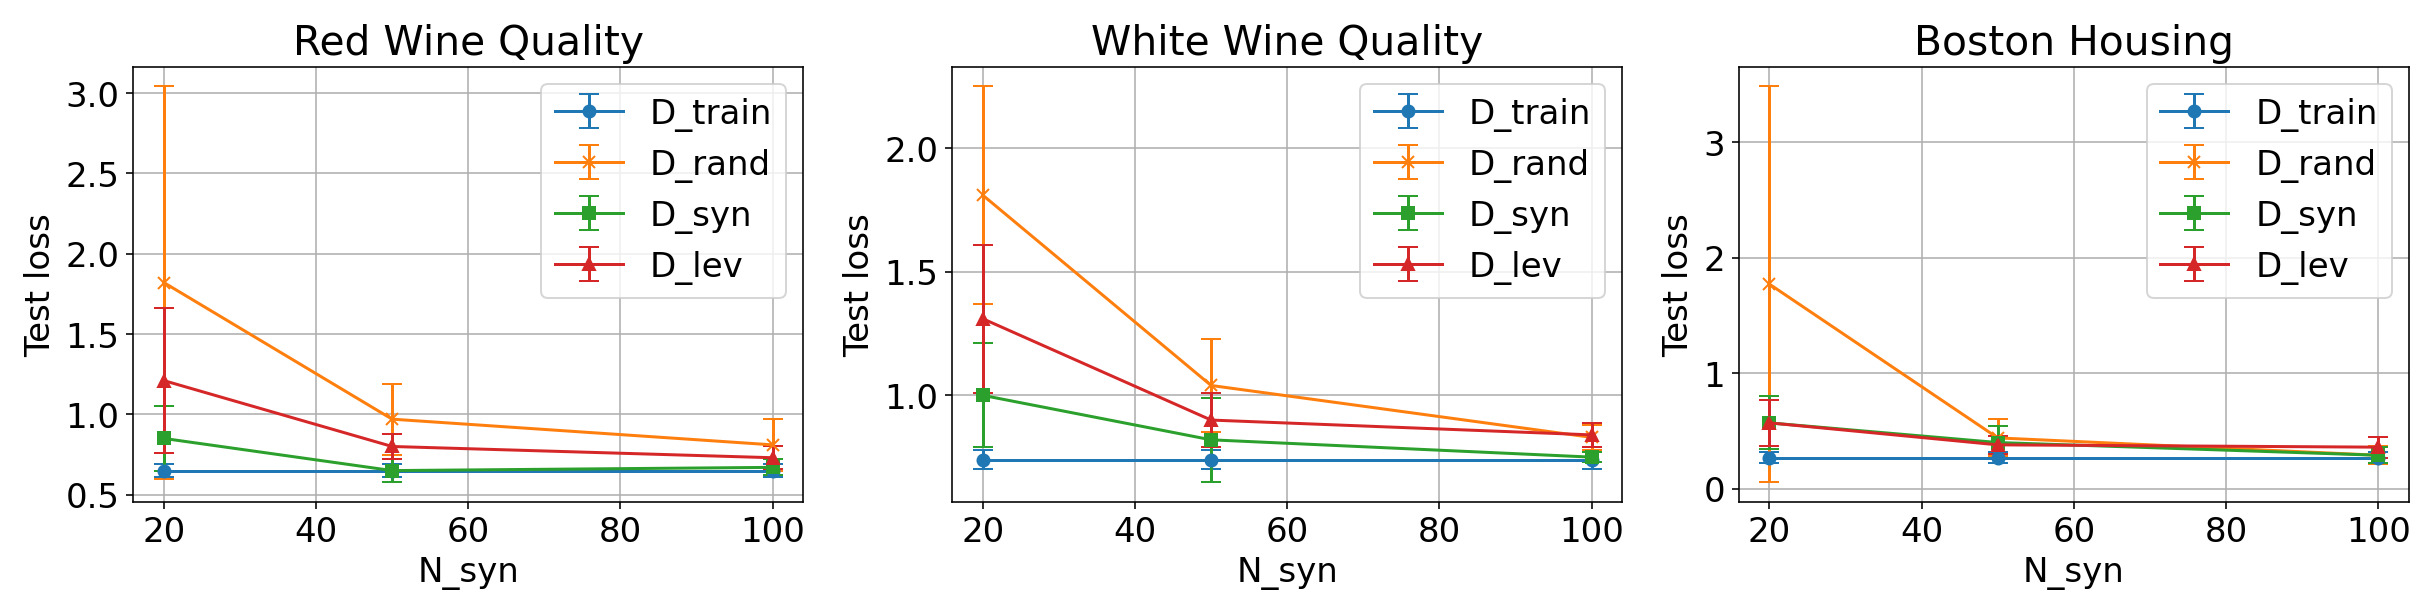
\includegraphics[width=\textwidth]{supervisedfinal.jpg}
	\caption{MSE Test losses for Homogeneous Linear Regression on the following supervised datasets: \it{red wine quality, white wine quality, Boston Housing}.}
    \label{fig:supervised}
\end{figure}
\begin{figure}
	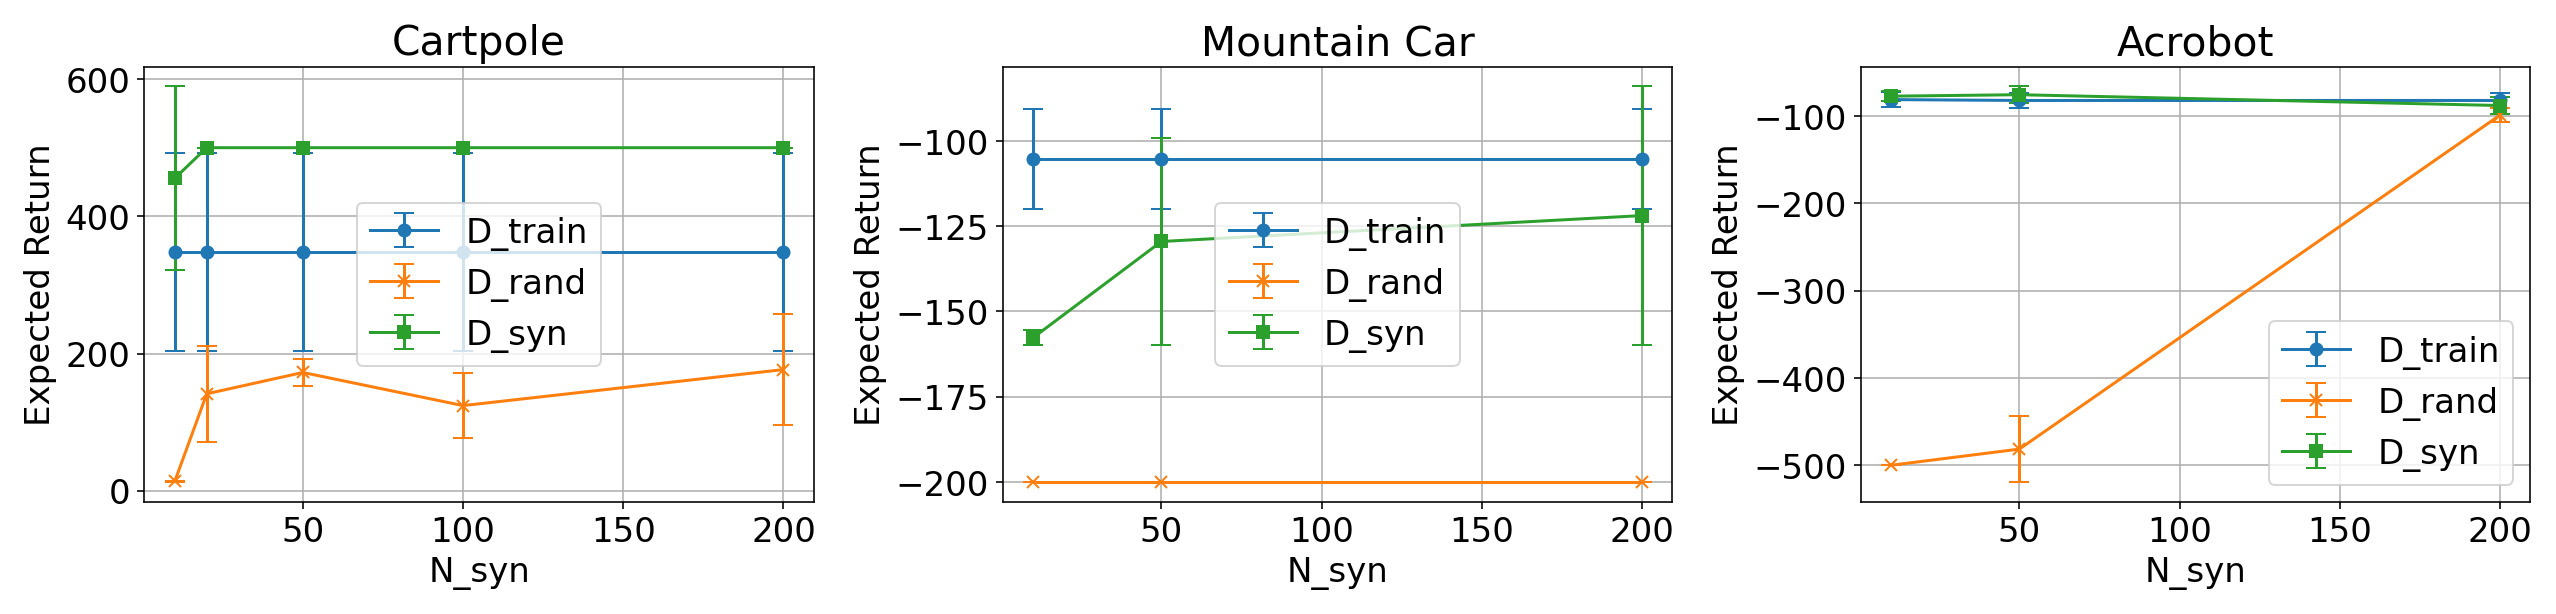
\includegraphics[width=\textwidth]{offlinerlfinal.jpg}
	\caption{Max Evaluation Return with two-layer neural networks on the offline RL datasets created by the following environments: \it{Cartpole, Mountain Car, Acrobot}.}
    \label{fig:offlinerl}
\end{figure}
Additional discussions and experimental evaluations are included in Appendix \ref{app:experiments}.\\


\section{Conclusions}
We propose a loss matching based algorithm for supervised dataset distillation, in which given a training dataset the synthetic dataset is optimized with respect to a fixed set of randomly sampled models. For linear regression in $\R^d$, we prove rigorous theoretical guarantees, showing that optimizing the convex loss matching objective for only $\tilde{O}(d^2)$ sampled regressors, without any model training, suffices to obtain a high quality synthetic dataset. We prove a matching lower bound of $\Omega(d^2)$ many sampled regressors, showing the tightness of our analysis. We extend our approach to offline RL to provide an algorithm for dataset distillation matching Bellman Loss using sampled $Q$-value predictors, while showing similar performance bounds, albeit requiring $\tn{exp}(O(d\log d))$ sampled predictors in the worst case. However, under a natural decomposability assumption on $d$-dimensional state-action embeddings, we improve the upper bound to $\tilde{O}(d^2)$. Our experiments show that our algorithms yield performance gains on real datasets, both in terms of the size and quality of the synthetic dataset, even with a small number of sampled predictors. 

An interesting yet challenging future direction in to extend our theoretical results in the supervised setting to neural networks, and to obtain provably efficient offline RL dataset distillation algorithms for more general classes of state-action embeddings, perhaps leveraging specific geometric properties of the associated MDPs.
